\chapter{Thực nghiệm và thảo luận}

\section{Phạm vi suy luận thực nghiệm}

Để hỗ trợ điều khiển, một biểu diễn tiến độ cần thỏa mãn ba điều kiện: có thể suy ra từ quan sát khả dụng, đến được chính sách đúng lúc và chứa thông tin mà chính sách có thể sử dụng để chọn hành động. Khóa luận xem xét ba loại bằng chứng: sự phù hợp của sự kiện với mốc tiến độ trong các quỹ đạo thao tác mẫu, độ nhạy của sai số dự đoán hành động đối với đầu vào bộ nhớ, và kết quả điều khiển vòng kín. Đối chiếu ba phép đo giúp xác định mắt xích nào đã có bằng chứng và mắt xích nào cần một phép can thiệp riêng.

Nguồn phân tích chính gồm phép phát lại sáu quỹ đạo thao tác mẫu ngày 26/10/2026, nhật ký xác thực của mô hình F1 và 40 quỹ đạo điều khiển hoàn tất trong đợt đánh giá ngày 09/11/2026. Với đợt đánh giá vòng kín, số liệu được tính lại từ từng bản tóm tắt quỹ đạo, sau khi đối chiếu tổng kiểm, trạng thái hoàn tất, tác vụ, trạng thái khởi tạo và hạt giống. Danh mục dữ liệu, phiên bản và tổng kiểm được lưu cùng bản ghi thực nghiệm ngày 12/11/2026 \cite{artifact2026}.

Đối chứng của phân tích vòng kín là B0 trên chính T1/T3. Kết quả V1 trong phụ lục chỉ cung cấp bối cảnh về chính sách gốc trên các tác vụ khác và với nhịp truy vấn khác. \cite{artifact2026}

\section{Mức phù hợp giữa sự kiện thị giác và mốc tiến độ}

Để khảo sát RQ2, bộ ghi sự kiện từ RGB được áp dụng trên sáu quỹ đạo thao tác mẫu T1/T3, gồm 1.276 khung hình và ba trạng thái khởi tạo. Với mỗi trạng thái đều có quỹ đạo của cả T1 lẫn T3. Hai quỹ đạo được dùng để phát triển phương pháp và các quỹ đạo bổ sung cũng đã được quan sát trước khi tổng hợp. Phép đo này vì vậy có phạm vi chẩn đoán trên những quỹ đạo đã biết. Nhãn tham chiếu mô tả thời điểm tiến độ tích lũy đạt mốc, nên phù hợp để đối chiếu sự kiện hoàn thành chu kỳ, còn thời điểm tiếp xúc hoặc nhả vật cần một loại nhãn khác.

Mỗi sự kiện đặt lại do bộ ghi xác nhận được ghép với nhiều nhất một mốc tham chiếu, trong dung sai 20 khung hình. Tất cả 12 sự kiện xác nhận đều ghép được với 12 mốc. Độ trễ xác nhận có trung vị 9 khung hình, trung bình xấp xỉ 9,92 khung hình và nằm trong khoảng 6–20 khung hình. Kết quả cho thấy có thể trích xuất một biến tiến độ hữu ích để mô tả những quỹ đạo đã xem từ bằng chứng thị giác. Độ trễ quan sát được cho thấy giữa thời điểm tiến độ thay đổi và thời điểm chính sách có thể nhận bằng chứng về thay đổi đó tồn tại một khoảng chờ cần tính đến.

\begingroup\small\setlength{\tabcolsep}{4pt}\renewcommand{\arraystretch}{1.15}
\begin{longtable}{>{\raggedright\arraybackslash}p{\dimexpr 0.25\textwidth-2\tabcolsep\relax}>{\raggedright\arraybackslash}p{\dimexpr 0.35\textwidth-2\tabcolsep\relax}>{\raggedright\arraybackslash}p{\dimexpr 0.4\textwidth-2\tabcolsep\relax}}
\caption{Đối chiếu sự kiện thị giác với mốc tiến độ trên các quỹ đạo mẫu}\label{tab:generated4}\\
\toprule
\textbf{Đại lượng khảo sát} & \textbf{Kết quả quan sát} & \textbf{Phạm vi diễn giải} \\
\midrule\endfirsthead
\toprule
\textbf{Đại lượng khảo sát} & \textbf{Kết quả quan sát} & \textbf{Phạm vi diễn giải} \\
\midrule\endhead
\bottomrule\endfoot
Quỹ đạo mẫu / trạng thái / khung hình & 6 / 3 / 1.276 & Các quỹ đạo hoàn thành tác vụ đã được quan sát \\
Mốc tham chiếu / sự kiện xác nhận / cặp ghép & 12 / 12 / 12 & Ghép một-một trong dung sai ±20 khung hình \\
Sự kiện dư / mốc bị bỏ sót & 0 / 0 & Tính trên sáu quỹ đạo mẫu \\
Độ trễ xác nhận & Trung vị 9, khoảng 6–20 khung hình & So với mốc tham chiếu \\
Phát hiện bát có IoU $\geq0{,}5$ & 1.169/1.172 (99,74\%) & Mẫu số chỉ gồm phát hiện đã được bộ theo dõi chấp nhận \\
Có định vị vật / có văn bản bộ nhớ & 1.172/1.276 / 1.258/1.276 khung hình & Tỷ lệ có đầu ra ở từng khâu \\
Lời nhắc dài nhất & 31 trên giới hạn 48 token & Đo bằng bộ tách token đã chọn \\
Độ trễ xử lý RGB & Khoảng 999–1.058 ms/khung hình & Độ trễ tính toán ở lần đo riêng \\
\end{longtable}
\endgroup

Tỷ lệ khớp hộp giới hạn đo chất lượng định vị có điều kiện trên các phát hiện được chấp nhận. Tỷ lệ này bỏ qua các khung mà đối tượng bị bỏ sót hoặc bị từ chối. Tương tự, việc tạo được văn bản chỉ chứng tỏ biểu diễn có đầu ra tại khung hình đó. Muốn ước lượng mức phù hợp của nội dung bộ nhớ trên phân phối điều khiển, cần cả quỹ đạo thành công lẫn thất bại và nhãn độc lập cho những tình huống như nhấc hụt, đặt lệch đĩa hoặc che khuất kéo dài.

Phụ lục ghi nguồn dữ liệu, phương pháp đối chiếu và các phép kiểm tính nhất quán của quá trình tạo bản ghi. \cite{artifact2026}

\section{Điều kiện đối chiếu trong mô phỏng}

Việc so sánh vòng kín giữa các chính sách đòi hỏi giữ ổn định động lực học, điều kiện quan sát và tiêu chí chấm điểm. Mức độ quy kết còn phụ thuộc vào những thành phần được thay đổi trong phép đối chứng. Hai lần chạy B0/F1 có cùng tổng kiểm của mô hình gốc, cấu hình đánh giá và danh sách trạng thái. Bản ghi nguồn của hai lần chạy khác nhau ở ba tập lệnh khởi chạy hoặc chẩn đoán. Các điểm khớp giúp thu hẹp diễn giải về biến gây nhiễu, còn khác biệt nguồn đặt giới hạn cho phát biểu về độ tương đương của hai lần chạy. Phụ lục mô tả quy trình đối chiếu bản ghi \cite{artifact2026}.

\begingroup\small\setlength{\tabcolsep}{4pt}\renewcommand{\arraystretch}{1.15}
\begin{longtable}{>{\raggedright\arraybackslash}p{\dimexpr 0.31\textwidth-2\tabcolsep\relax}>{\raggedright\arraybackslash}p{\dimexpr 0.69\textwidth-2\tabcolsep\relax}}
\caption{Các điều kiện đối chiếu trong thực nghiệm vòng kín}\label{tab:generated5}\\
\toprule
\textbf{Điều kiện} & \textbf{Giá trị dùng trong thực nghiệm} \\
\midrule\endfirsthead
\toprule
\textbf{Điều kiện} & \textbf{Giá trị dùng trong thực nghiệm} \\
\midrule\endhead
\bottomrule\endfoot
Mô hình gốc & SmolVLA cho LIBERO, cùng phiên bản ở B0 và F1 \\
Nguồn tác vụ và bộ chấm & LIBERO-Mem tại phiên bản đã khóa \\
Mô phỏng & Franka Panda trong robosuite 1.4.0, cùng thiết lập động lực học \\
Đầu vào chính sách & Hai camera 256×256, trạng thái 8 chiều, tiền xử lý theo checkpoint gốc \\
Điều khiển & OSC\_POSE ở 20 Hz trong mô phỏng, dự đoán $H=50$, thực thi $s=10$ \\
Khởi tạo và điểm cuối & Trạng thái từ danh sách đã khóa, 20 bước làm ấm, tối đa 1.000 hành động chính sách, dừng sớm khi vượt số chu kỳ \\
\end{longtable}
\endgroup

Huấn luyện sử dụng hai GPU Tesla T4. Phép đánh giá dùng NVIDIA GeForce RTX 4060 Laptop, với mô phỏng chạy trong WSL và suy luận chính sách trên Windows. Những điều kiện này xác định môi trường áp dụng của kết quả. Chu kỳ danh định 20 Hz của bộ điều khiển tương ứng 50 ms mỗi bước mô phỏng. Riêng thời gian xử lý một khung hình RGB trong phép đo chẩn đoán đã xấp xỉ một giây. Thời gian phát lại máy trạng thái từ dữ liệu đã lưu khoảng 1–2 ms mỗi khung hình phản ánh chi phí của một thành phần khác, sau khi đã có kết quả nhận dạng vật. Khi mô phỏng tạm dừng để chờ suy luận, tiến độ mô phỏng và thời gian thực trôi qua là hai đại lượng khác nhau. Một kết luận về khả năng vận hành thời gian thực cần đo trọn chu trình trên cấu hình đã xác định.

\section{Mẫu nghiên cứu và điều kiện thích ứng}

Tập dữ liệu huấn luyện kết hợp quỹ đạo thao tác cơ sở LIBERO-10 với quỹ đạo T1/T3 từ nguồn LIBERO-Mem của tác giả. Bảng dưới ghi số quỹ đạo trong danh mục dữ liệu được dùng để huấn luyện F1. Các quỹ đạo có cùng mã băm trạng thái khởi tạo được phân vào cùng một tập. Trong tập kiểm tra T1/T3, 20 tổ hợp tác vụ và trạng thái của mỗi điều kiện tương ứng 10 nhóm trạng thái dùng chung giữa hai tác vụ. Tập này đã được sử dụng trong quá trình phát triển. Vì vậy, số liệu vòng kín phù hợp cho phân tích thăm dò và hình thành giả thuyết kiểm chứng.

\begingroup\small\setlength{\tabcolsep}{4pt}\renewcommand{\arraystretch}{1.15}
\begin{longtable}{>{\raggedright\arraybackslash}p{\dimexpr 0.29\textwidth-2\tabcolsep\relax}>{\raggedright\arraybackslash}p{\dimexpr 0.1775\textwidth-2\tabcolsep\relax}>{\raggedright\arraybackslash}p{\dimexpr 0.1775\textwidth-2\tabcolsep\relax}>{\raggedright\arraybackslash}p{\dimexpr 0.1775\textwidth-2\tabcolsep\relax}>{\raggedright\arraybackslash}p{\dimexpr 0.1775\textwidth-2\tabcolsep\relax}}
\caption{Phân hoạch quỹ đạo theo nhóm tác vụ}\label{tab:generated6}\\
\toprule
\textbf{Nhóm dữ liệu} & \textbf{Huấn luyện} & \textbf{Xác thực} & \textbf{Kiểm tra} & \textbf{Tổng} \\
\midrule\endfirsthead
\toprule
\textbf{Nhóm dữ liệu} & \textbf{Huấn luyện} & \textbf{Xác thực} & \textbf{Kiểm tra} & \textbf{Tổng} \\
\midrule\endhead
\bottomrule\endfoot
Thao tác cơ sở LIBERO-10 & 400 & 50 & 50 & 500 \\
Mem T1 & 80 & 10 & 10 & 100 \\
Mem T3 & 78 & 10 & 10 & 98 \\
Tổng & 558 & 70 & 70 & 698 \\
\end{longtable}
\endgroup

Lấy mẫu hỗn hợp nhằm đặt ra bài toán duy trì kỹ năng cơ sở (RQ3) trong cùng quá trình thích ứng với tác vụ phụ thuộc lịch sử. Trong mỗi lô cập nhật, số mẫu của hai miền được phân bổ theo tỷ lệ đã chọn. Trong từng miền, tác vụ được chọn luân phiên, sau đó lấy mẫu đều theo quỹ đạo rồi chọn khung hình. Cách này làm giảm ảnh hưởng của độ dài quỹ đạo lên xác suất được chọn. Tỷ lệ lấy mẫu 50/50 là một điều kiện huấn luyện đã quan sát, nên giá trị của việc trộn dữ liệu và lựa chọn tỷ lệ vẫn cần đối chứng riêng.

\begingroup\small\setlength{\tabcolsep}{4pt}\renewcommand{\arraystretch}{1.15}
\begin{longtable}{>{\raggedright\arraybackslash}p{\dimexpr 0.18\textwidth-2\tabcolsep\relax}>{\raggedright\arraybackslash}p{\dimexpr 0.23\textwidth-2\tabcolsep\relax}>{\raggedright\arraybackslash}p{\dimexpr 0.26\textwidth-2\tabcolsep\relax}>{\raggedright\arraybackslash}p{\dimexpr 0.33\textwidth-2\tabcolsep\relax}}
\caption{Cấu hình thích ứng của F1 và phạm vi suy luận}\label{tab:generated7}\\
\toprule
\textbf{Hạng mục} & \textbf{Cấu hình đã sử dụng} & \textbf{Vai trò nghiên cứu} & \textbf{Giới hạn suy luận} \\
\midrule\endfirsthead
\toprule
\textbf{Hạng mục} & \textbf{Cấu hình đã sử dụng} & \textbf{Vai trò nghiên cứu} & \textbf{Giới hạn suy luận} \\
\midrule\endhead
\bottomrule\endfoot
Vị trí thích ứng & LoRA tại phép chiếu query/value của khối sinh hành động, hạng 16, 645.120 tham số được cập nhật & Giữ mô hình nền cố định khi thích ứng & Chỉ khảo sát một vị trí và một hạng \\
Tối ưu hóa & AdamW, tốc độ học ban đầu $2\times10^{-5}$, làm ấm 100 bước, 3.000 bước cập nhật, chặn chuẩn gradient 1,0 & Cố định ngân sách của F1 & Chưa có khảo sát siêu tham số \\
Lấy mẫu hỗn hợp & Lô hiệu dụng 32, tỷ lệ dữ liệu cơ sở 0,5, hạt giống 42 & Đặt kỹ năng cơ sở và thích ứng vào cùng bài toán huấn luyện & Mức độ duy trì cần đo bằng điều khiển vòng kín \\
Bộ nhớ khi huấn luyện & Tỷ lệ bỏ bộ nhớ bằng 0, xác thực và lưu mô hình mỗi 500 bước & Xác định phân phối đầu vào của F1 & Bỏ bộ nhớ khi suy luận có thể thay đổi phân phối \\
Mô hình được đánh giá & Trọng số LoRA lưu riêng, dùng checkpoint ở bước 3.000 & Cố định phiên bản dùng cho các phép đo & Chưa chọn checkpoint theo tỷ lệ thành công vòng kín \\
\end{longtable}
\endgroup

Tổng kiểm của danh mục dữ liệu khớp với bản ghi huấn luyện, và bốn tệp được liệt kê trong bản xuất F1 có tổng kiểm khớp bản kê. Phép đối chiếu giới hạn ở các tệp đã nêu. Dữ liệu Mem của F1 dùng các quỹ đạo do tác giả công bố, với ảnh được đưa về quy ước gốc trước khi áp dụng tiền xử lý của chính sách. Một đợt tái tạo dữ liệu tại chỗ ghi nhận 73 trên 78 quỹ đạo phát lại T3 đạt điều kiện thành công của đợt phát lại. Các quỹ đạo đó là một nhánh nghiên cứu riêng. Chuỗi xác thực dữ liệu dẫn xuất, lập chỉ mục và huấn luyện trên phiên bản derived-v1 chưa hoàn tất, nên phân tích F1 căn cứ vào tập dữ liệu của tác giả \cite{artifact2026}.

\section{Độ nhạy ngoại tuyến đối với thông tin bộ nhớ}

Tại bước 3.000, trên 4.299 mẫu khung hình của tập xác thực Mem, hàm mất mát flow matching của cùng F1 là 0,23023575 khi có bộ nhớ và 0,33553660 khi bỏ bộ nhớ. Trên 13.525 mẫu khung hình của tập xác thực cơ sở, hai chế độ đều cho giá trị 0,42984212. Các khung hình được lấy từ quỹ đạo và có thể phụ thuộc theo thời gian. Phép so sánh giữ cố định trọng số F1 và thay đổi cách cung cấp bộ nhớ ở đầu vào.

\begin{figure}[htbp]
\centering
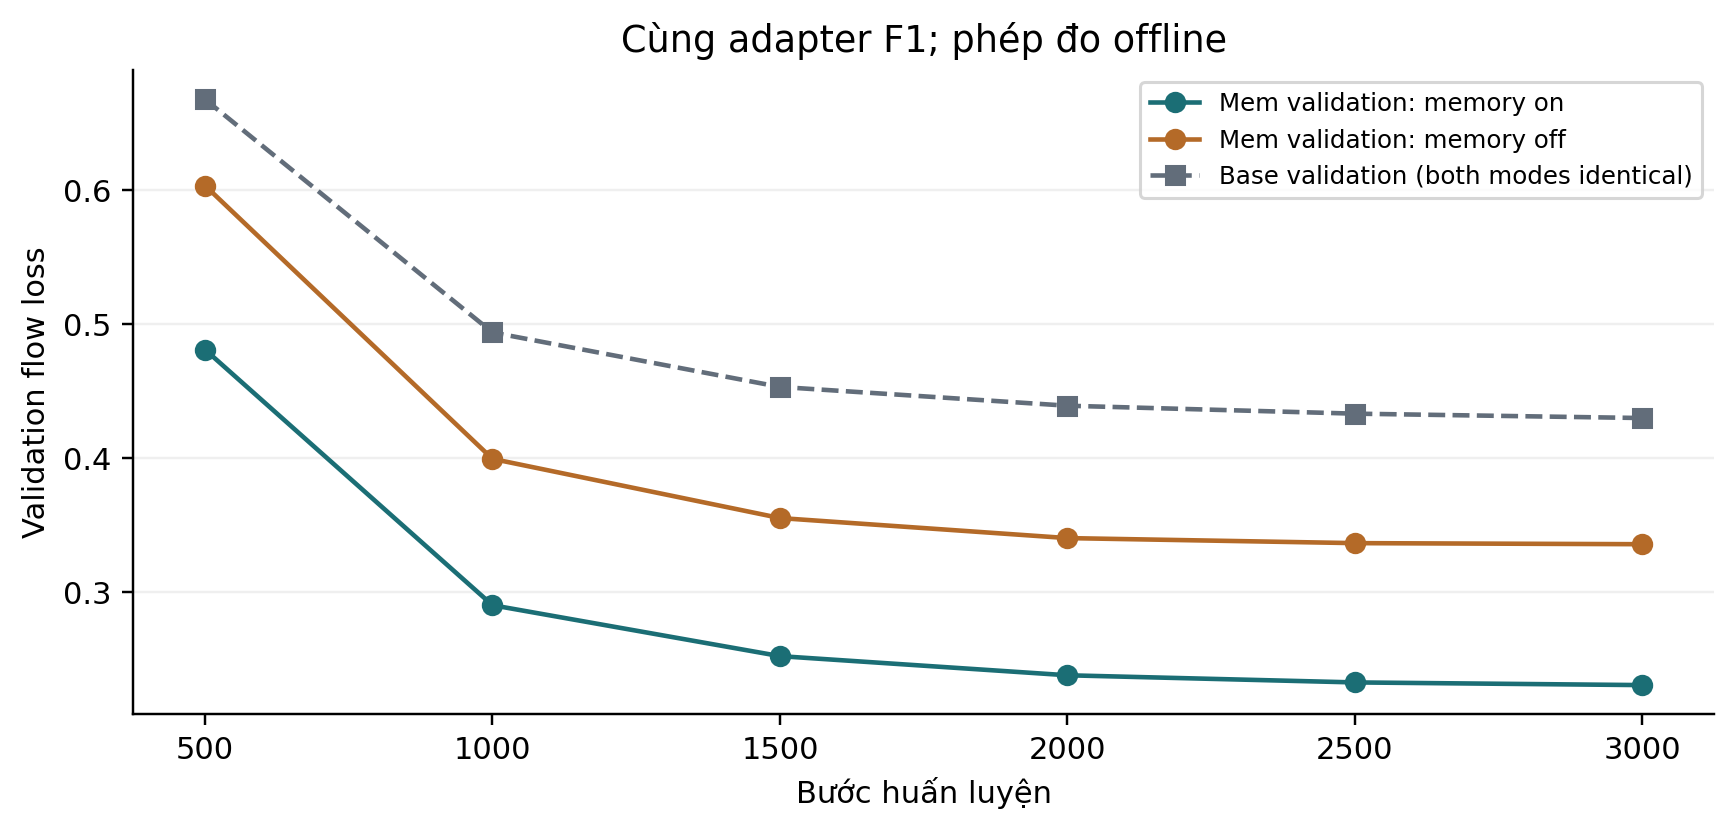
\includegraphics[width=\textwidth]{../figures/validation_loss.png}
\caption{Hàm mất mát flow matching trên tập xác thực theo số bước huấn luyện. Hai chế độ có và bỏ bộ nhớ được đo trên cùng checkpoint ở mỗi bước.}
\label{fig:validation_loss}
\end{figure}

Chênh lệch trên tập Mem là bằng chứng rằng cách cung cấp đầu vào bộ nhớ có liên hệ với chất lượng dự đoán hành động trên phân phối xác thực. Do F1 được huấn luyện với tỷ lệ bỏ bộ nhớ bằng 0, phép bỏ bộ nhớ có thể đồng thời loại thông tin tiến độ và đưa đầu vào ra ngoài phân phối huấn luyện. Để tách hai cách giải thích này, một phép thử có kiểm soát cần duy trì định dạng và dung lượng lời nhắc, đồng thời thay đổi có chủ đích thông tin lịch sử mà nó chứa. Mặt khác, một chính sách có sai số dự đoán nhỏ trên các quỹ đạo thao tác mẫu vẫn có thể thực thi kém khi các hành động của chính nó làm thay đổi phân phối quan sát.

Về khả năng duy trì kỹ năng trong RQ3, hai giá trị hàm mất mát bằng nhau trên tập cơ sở chỉ phản ánh tính ổn định giữa hai chế độ đầu vào của F1 trong phép đo này. Chẳng hạn, các mẫu cơ sở có thể có cùng đầu vào ở hai chế độ nếu chúng đều không mang hậu tố bộ nhớ. Để ước lượng mức duy trì kỹ năng, phép so sánh cần đặt chính F1 và B0 vào cùng các tác vụ cơ sở, với tiêu chí thành công và ngân sách điều khiển giống nhau.

\section{Kết quả điều khiển vòng kín}

RQ1 đặt vấn đề liệu lịch sử có giúp chính sách hoàn thành tác vụ khi đã kiểm soát thích ứng mô hình. Dữ liệu hiện có đối chiếu B0, tức checkpoint gốc, với F1, tức cấu hình có cả thích ứng và bộ nhớ quan sát trực tuyến. Đây là phép so sánh sơ bộ hai cấu hình nghiên cứu. Mỗi điều kiện dùng cùng 20 tổ hợp tác vụ và trạng thái, với hạt giống chính sách 42. Kết quả áp dụng cho giao thức T1/T3 của khóa luận, với nhãn \path{CUSTOM_V2_LIBERO_MEM} và \path{NON-COMPARABLE_OFFICIAL_PAPER}.

\begingroup\small\setlength{\tabcolsep}{4pt}\renewcommand{\arraystretch}{1.15}
\begin{longtable}{>{\raggedright\arraybackslash}p{\dimexpr 0.12\textwidth-2\tabcolsep\relax}>{\raggedright\arraybackslash}p{\dimexpr 0.14\textwidth-2\tabcolsep\relax}>{\raggedright\arraybackslash}p{\dimexpr 0.2\textwidth-2\tabcolsep\relax}>{\raggedright\arraybackslash}p{\dimexpr 0.12\textwidth-2\tabcolsep\relax}>{\raggedright\arraybackslash}p{\dimexpr 0.19\textwidth-2\tabcolsep\relax}>{\raggedright\arraybackslash}p{\dimexpr 0.23\textwidth-2\tabcolsep\relax}}
\caption{Kết quả điều khiển vòng kín theo tác vụ và điều kiện}\label{tab:generated8}\\
\toprule
\textbf{Nhiệm vụ} & \textbf{Điều kiện} & \textbf{Thành công / số lượt} & \textbf{SR} & \textbf{SCR trung bình} & \textbf{Vượt số chu kỳ / số lượt} \\
\midrule\endfirsthead
\toprule
\textbf{Nhiệm vụ} & \textbf{Điều kiện} & \textbf{Thành công / số lượt} & \textbf{SR} & \textbf{SCR trung bình} & \textbf{Vượt số chu kỳ / số lượt} \\
\midrule\endhead
\bottomrule\endfoot
T1 & B0 & 0/10 & 0\% & 0,1000 & 1/10 \\
T1 & F1 & 0/10 & 0\% & 0,1000 & 1/10 \\
T3 & B0 & 0/10 & 0\% & 0,0000 & 0/10 \\
T3 & F1 & 1/10 & 10\% & 0,1667 & 0/10 \\
Hai tác vụ & B0 & 0/20 & 0\% & 0,0500 & 1/20 \\
Hai tác vụ & F1 & 1/20 & 5\% & 0,1333 & 1/20 \\
\end{longtable}
\endgroup

\begin{figure}[htbp]
\centering
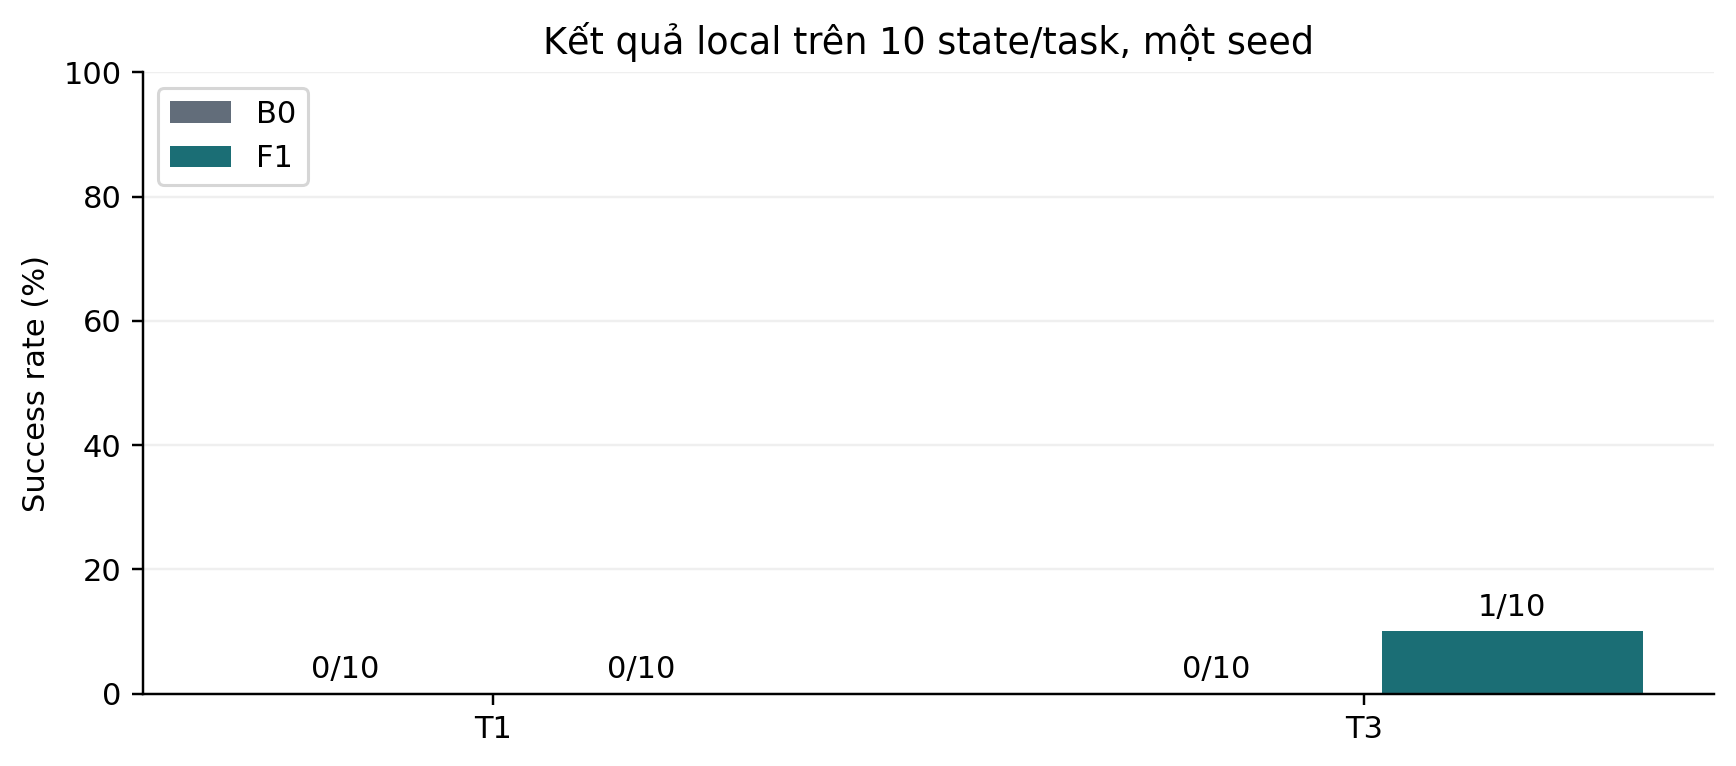
\includegraphics[width=\textwidth]{../figures/mem_success.png}
\caption{Tỷ lệ thành công trên T1 và T3 theo giao thức của khóa luận. Mỗi cột biểu diễn 10 quỹ đạo. Hai tác vụ dùng chung các nhóm trạng thái khởi tạo và cùng một hạt giống chính sách.}
\label{fig:mem_success}
\end{figure}

Gọi $S_{c,j}$ là chỉ báo thành công của điều kiện $c$ trên tổ hợp tác vụ và trạng thái thứ $j$. Chênh lệch tỷ lệ thành công quan sát được tính theo

\begin{equation}
\widehat{\Delta}_{\mathrm{SR}}
=\frac{1}{M}\sum_{j=1}^{M}\left(S_{F1,j}-S_{B0,j}\right),
\qquad M=20.
\end{equation}

Có 19 cặp có kết quả $(0,0)$ và một cặp có kết quả $(0,1)$ theo thứ tự $(B0,F1)$, nên $\widehat{\Delta}_{\mathrm{SR}}=0{,}05$, tức 5 điểm phần trăm. Toàn bộ chênh lệch đến từ một lần thực thi T3. Hai tác vụ chia sẻ 10 nhóm trạng thái và thí nghiệm chỉ dùng một hạt giống, nên báo cáo giới hạn ở thống kê mô tả. Việc ước lượng độ bất định cần thêm biến thiên qua trạng thái và hạt giống, đồng thời giữ cấu trúc ghép cặp.

SCR ghi nhận mức hoàn thành từng phần. Trên T1, cả B0 và F1 đều có một quỹ đạo đạt mốc tiến độ nhưng tiếp tục đến mức vượt số chu kỳ. Trên T3, SCR trung bình của F1 là 0,1667 trong khi của B0 bằng 0, cho thấy bộ đánh giá ghi nhận thêm tiến độ ở một số lần chạy. Diễn giải này bổ sung cho tỷ lệ thành công, vì tiến độ từng phần và hoàn thành ở điểm cuối là hai tiêu chí khác nhau. Đối chứng F0 thích ứng trên cùng dữ liệu nhưng không có bộ nhớ và phép đánh giá F1 khi thay đổi có kiểm soát đầu vào lịch sử vẫn cần thiết để trả lời RQ1.

\section{Bất đồng giữa tiến độ quan sát và tiến độ được chấm}

Khi chính sách tự sinh quỹ đạo, nó có thể đưa hệ thống đến những tình huống ít gặp trong dữ liệu thao tác mẫu. Trên 20 quỹ đạo F1, 19 trạng thái bộ nhớ cuối báo lịch sử chưa đầy đủ. Trong 1.927 lần gọi chính sách, 1.894 lời nhắc chứa hậu tố bộ nhớ và 1.738 lời nhắc chứa cụm \path{history incomplete}. Hai số đếm ở cấp lời nhắc lần lượt phản ánh tần suất cung cấp bộ nhớ và tần suất báo lịch sử chưa đầy đủ. Chúng là các phép đo lặp theo thời gian trên cùng quỹ đạo. Độ đúng của từng sự kiện đòi hỏi đối chiếu với nhãn độc lập.

Quỹ đạo T3 thành công duy nhất của F1 là một trường hợp chẩn đoán cho RQ2. Tại bước 1.000, bộ đánh giá ghi đủ ba chu kỳ, điều kiện cuối được thỏa mãn và số chu kỳ không bị vượt. Bộ ghi thị giác cuối chỉ xác nhận hai lần đặt lại và đánh dấu lịch sử chưa đầy đủ. Bất đồng này làm suy yếu cách giải thích rằng chính sách dừng khi bộ đếm thị giác ghi đủ ba chu kỳ. Kết quả vẫn tương thích với nhiều cơ chế, chẳng hạn sử dụng một phần bằng chứng lịch sử, phản ứng với quan sát hiện tại, hoặc hành vi đã thay đổi qua thích ứng trọng số.

Trong lượt T1 của F1 bị vượt số chu kỳ, bộ đánh giá ghi một mốc và SCR bằng 1, nhưng dừng quỹ đạo tại bước 266 do vượt số chu kỳ. Bộ ghi thị giác cuối ghi nhận 0 lần đặt lại và lịch sử chưa đầy đủ. B0 cũng có một quỹ đạo T1 vượt số chu kỳ, ở trạng thái 3 và bước 290. Những trường hợp này chỉ ra hai vấn đề khác nhau: hệ thống có thể thực hiện thao tác đạt mốc nhưng không duy trì đúng điểm cuối, và bộ ghi thị giác có thể thiếu bằng chứng để xác nhận mốc mà bộ đánh giá đã ghi nhận. Muốn quy nguyên nhân cần nhãn độc lập theo thời gian và can thiệp riêng lên nội dung bộ nhớ trong khi giữ các điều kiện còn lại ổn định.

\section{Hiệu lực của kết luận và thiết kế kiểm chứng tiếp theo}

Đối với RQ2, sự phù hợp trong sáu quỹ đạo mẫu cung cấp bằng chứng về tính khả thi của việc biểu diễn tiến độ bằng sự kiện thị giác. Dấu thời điểm khả dụng cho phép kiểm tra dữ kiện nào đã có thể đưa vào lời nhắc tại từng bước. Khoảng cách giữa kết quả ghép mốc trên quỹ đạo mẫu và tỷ lệ lịch sử chưa đầy đủ trên quỹ đạo F1 đặt ra giới hạn về tính đại diện của phép kiểm chẩn đoán. Một tập nhãn độc lập gồm cả tình huống thất bại, với quy tắc ghép và dung sai đặt trước, cho phép ước lượng riêng xác nhận sai, bỏ sót, độ trễ và tỷ lệ tình huống chưa xác định.

Đối với RQ1, cần giữ dữ liệu, phân hoạch, ngân sách huấn luyện và quy tắc chọn checkpoint giống nhau khi so F0 với F1. Phép thử can thiệp lúc suy luận cần có điều kiện chỉ dùng thông tin hiện tại và điều kiện có cùng định dạng nhưng thay đổi giá trị lịch sử. Hai phép so sánh trả lời các câu hỏi khác nhau: thích ứng với bộ nhớ có tạo lợi ích vòng kín hay không, và chính sách đã thích ứng nhạy thế nào với nội dung cụ thể của bộ nhớ. Một tập trạng thái xác nhận độc lập với phát triển và nhiều hạt giống sẽ cho phép ước lượng chênh lệch ghép cặp cùng độ bất định ở cấp nhóm trạng thái. Chỉ đổi hạt giống trên các trạng thái đã dùng để phát triển không tạo một tập xác nhận độc lập.

Về khả năng duy trì kỹ năng trong RQ3, đánh giá chính F1 trên các tác vụ cơ sở ghép cặp với B0 là cách đo trực tiếp mức duy trì. Nếu mục tiêu là kiểm tra tính không kém hơn, cần xác định trước biên suy giảm có thể chấp nhận được và cỡ mẫu đủ để diễn giải biên đó. Cơ chế chọn lại trọng số B0 cho tác vụ cơ sở chỉ đo chất lượng của một quy tắc định tuyến và không định lượng kỹ năng của F1.

Đối với RQ2, ưu tiên can thiệp vào những yếu tố có thể đổi giá trị hoặc thời điểm khả dụng của bằng chứng, gồm quy ước ảnh, độ trễ xác nhận và số hành động giữa hai lần gọi chính sách. Có thể dùng cùng một quỹ đạo để kiểm tra tác động riêng lên chất lượng quan sát trước khi thay đổi các yếu tố đó trong vòng kín. Cần báo cáo cả thời gian mô phỏng và thời gian thực đo trên phần cứng. Thiết kế như vậy gắn mỗi phép đo với một cơ chế sai lệch cụ thể, từ sai số của biểu diễn cho đến hạn chế về cách sử dụng biểu diễn trong điều khiển.

